%                                                                 aa.dem
% AA vers. 9.1, LaTeX class for Astronomy & Astrophysics
% demonstration file
%                                                       (c) EDP Sciences
%-----------------------------------------------------------------------
%
%\documentclass[referee]{aa} % for a referee version
%\documentclass[onecolumn]{aa} % for a paper on 1 column  
%\documentclass[longauth]{aa} % for the long lists of affiliations 
%\documentclass[letter]{aa} % for the letters 
%\documentclass[bibyear]{aa} % if the references are not structured 
%                              according to the author-year natbib style

%
\documentclass{aa}  

%
\usepackage{graphicx}
\usepackage{float}
% \usepackage{algorithmic}
\usepackage[lined,ruled,linesnumbered,algoruled,french,commentsnumbered]{algorithm2e}
\usepackage{svg}
%%%%%%%%%%%%%%%%%%%%%%%%%%%%%%%%%%%%%%%%
\usepackage{txfonts}
%%%%%%%%%%%%%%%%%%%%%%%%%%%%%%%%%%%%%%%%
%\usepackage[options]{hyperref}
% To add links in your PDF file, use the package "hyperref"
% with options according to your LaTeX or PDFLaTeX drivers.
%
\begin{document} 


   \title{Tunable Kernel-Nulling for direct detection of exoplanets}

   \subtitle{1. Calibration and performance}

   \author{V. Foriel\inst{1},
            F. Martinache\inst{1},
            D. Mary\inst{1}
            \and
            R. Laugier\inst{2}
          }

   \institute{Université Côte d’Azur, Observatoire de la Côte d’Azur Nice, CNRS, Laboratoire Lagrange, Nice, France
         \and
            KU Leuven university, Leuven, Belgium
             }

   \date{Received ---; accepted ---}

% \abstract{}{}{}{}{} 
% 5 {} token are mandatory
 
  \abstract
  % context heading (optional)
  % {} leave it empty if necessary  
   {Lorem ipsum}
  % aims heading (mandatory)
   {Lorem ipsum}
  % methods heading (mandatory)
   {Lorem ipsum}
  % results heading (mandatory)
   {Lorem ipsum}
  % conclusions heading (optional), leave it empty if necessary 
   {Lorem ipsum}

   \keywords{Lorem ipsum}

   \maketitle
%
%-------------------------------------------------------------------

\section{Introduction}

    \begin{enumerate}
        \item Nulling interferometry
        \item Kernel nulling
        \item Integrated optics \& phase shifters
    \end{enumerate}

%--------------------------------------------------------------------

\section{Materials and conditions}

    \begin{enumerate}
        \item VLTI/ASGARD (/NOTT?)
        \item Integrated optics \& phase shifters
        \item Studied architecture
        \item Observation conditions (Vegga-like star, noise etc.)
    \end{enumerate}

\section{System modelisation \& calibration}
    \begin{enumerate}
        \item Calibration methods (Fig \ref{fig:perturbed_phases} \& \ref{fig:calibrated_phases})
        \subitem Genertic Algorithm
        \subitem Input obstruction
        \subitem Machine Leaning?
    \end{enumerate}

    \begin{figure}[H]
        \begin{center}
        \begin{tabular}{c}
        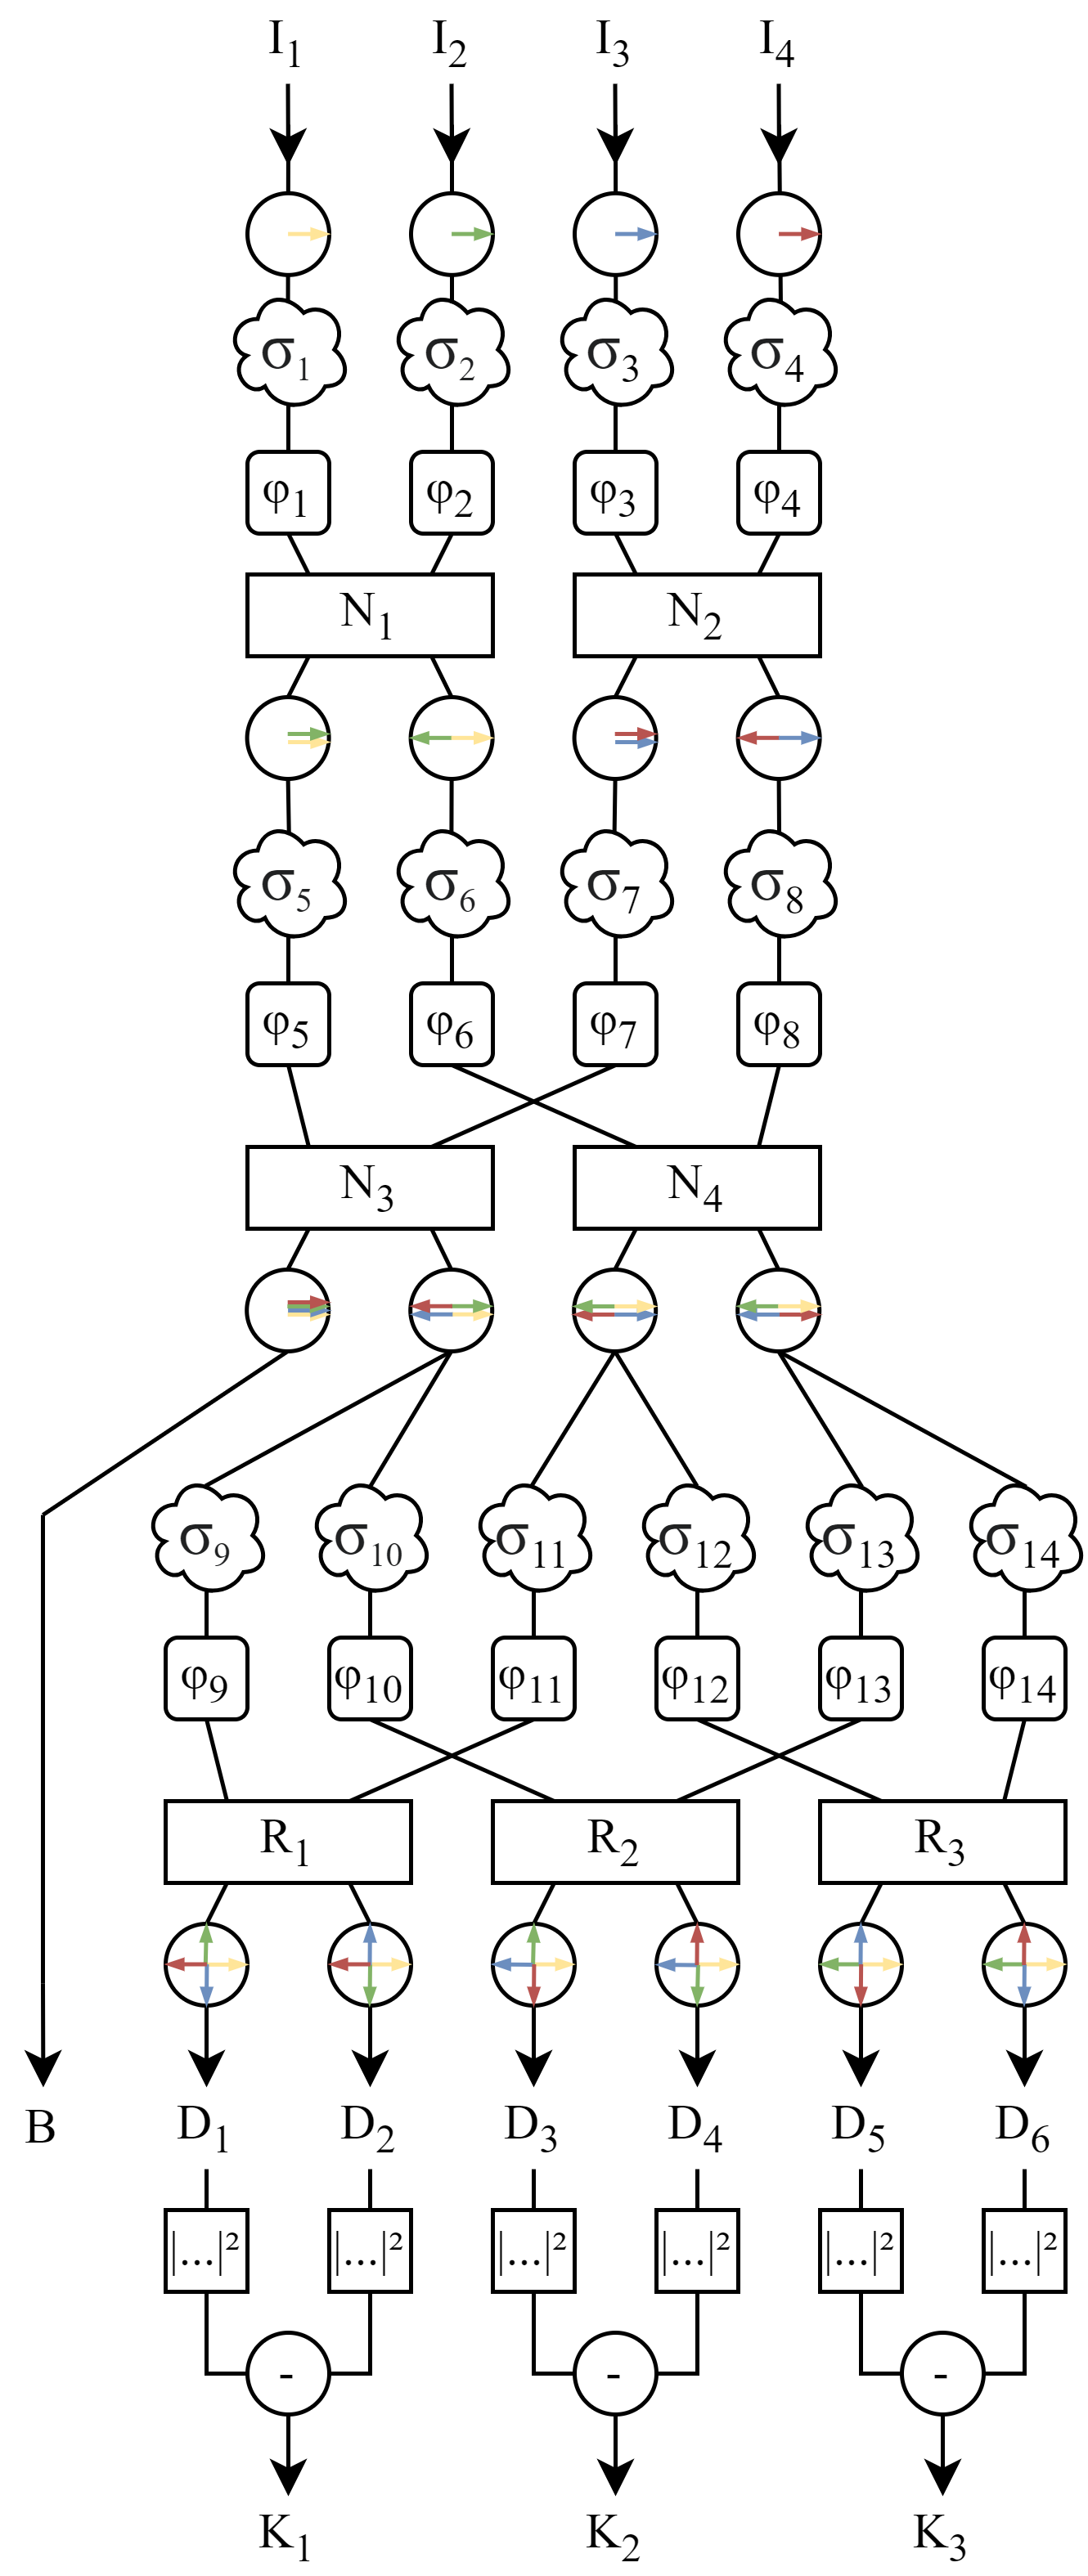
\includegraphics[width=8cm]{img/kernel_scheme.png}
        \end{tabular}
        \end{center}
        \caption[architecture] 
        { \label{fig:architecture} 
        Studied architecture}
    \end{figure}

    \subsection{Algorithms}

        In order to calibrate the component, two algorithms have been developed. The first is based on the principle of a genetic algorithm, the second on the principle of input obstruction. Both algorithms have been implemented in Python and are based on the same principle: we seek to optimize the component's performance by introducing phase variations on each phase shifter. The difference between the two algorithms lies in the way these phase variations are introduced and the metrics used to evaluate the component's performance. We will present both methods and discuss their advantages and limitations.

        Consistent with our architecture (Figure \ref{fig:architecture}), these algorithmes involve the following quantities:
        \begin{itemize}
            \item $I_n$ the $n^{th}$ input signal (electric field)
            \item $B$ the bright output signal (electric field)
            \item $D_n$ the $n^{th}$ dark output signal (electric field)
            \item $K_n$ the $n^{th}$ kernel output (intensity). We have:
            \subitem $K_1 = |D_1|^2 - |D_2|^2$
            \subitem $K_2 = |D_3|^2 - |D_4|^2$
            \subitem $K_3 = |D_5|^2 - |D_6|^2$
            \item $P_n$ the phase introduced on the $n^{th}$ phase shifter (distance)
        \end{itemize}

        \subsubsection{Genetic}
            The first algorithm that was developed is based on the principle of deterministic genetic algorithm. We define a performance metric $M$, which in this case corresponds to the kernel-null depth, then we seek to optimize it by successively introducing a phase variation $\Delta \phi$ on each phase shifter $P_n$.

            The optimization process is performed using a point source that simulates a single star. The goal is to nullify its signal on the dark outputs. However, since Kernels are constructed via the difference of two dark outputs, it is possible to obtain very good kernel-nulls without necessarily having well nullified the star's light. To address this issue, we define two different metrics, one measuring the average kernel-null depth $M_K$ that we want to minimize, the other measuring the intensity obtained on the bright output of the component $M_B$ (which is opposed to the total intensity obtained over all the dark outputs) that we want to maximize. Thus, we have:

            \begin{equation}
                M_K = \sum_{n=1}^3 K_n
            \end{equation}

            \begin{equation}
                M_B = |B|^2
            \end{equation}
            
            Given our component's architecture, we can associate the metric $M_B$ with each phase shifter that affects the bright output, namely $P_{1 \rightarrow 5}$ and $P_7$. All other phase shifters are then associated with the metric $M_K$ (cf. Algorithme \ref{genetic} line 3-4).

            The genetic algorithm is then structured as follows:

            \begin{algorithm}
            \caption{Genetic calibration algorithm}
            \label{genetic}
            \SetKwInOut{Input}{Inputs}\SetKwInOut{Output}{Output}
            
            \Input{$\varepsilon$: desired phase precision\\
                   $\beta$: phase variation reduction factor ($\beta \in [0.5,1[$)}
            \Output{$\vec{P}$: optimized phase shifts vector}
            \BlankLine
            
            $\vec{P} \leftarrow \vec{0}$ \tcp*{Initialize phase shifts to 0}
            $\Delta\phi \leftarrow \lambda/4$ \tcp*{Initial phase variation}
            $\vec{PM_B} \leftarrow [1,5] \cup [7]$ \tcp*{Phase shifters for bright output}
            $\vec{PM_K} \leftarrow [6] \cup [8,14]$ \tcp*{Phase shifters for kernel-nulls}
            \BlankLine
            
            \While{$\Delta\phi > \varepsilon$}{
                \For{$n \leftarrow 1$ \KwTo $14$}{
                    $\vec{P^+} \leftarrow \vec{P}$\;
                    $P^+_n \leftarrow P_n + \Delta\phi$\;
                    
                    $\vec{P^-} \leftarrow \vec{P}$\;
                    $P^-_n \leftarrow P_n - \Delta\phi$\;
                    
                    \uIf{$n \in \vec{PM_B}$}{
                        \If{$M_B(\vec{P^+}) > M_B(\vec{P})$}{
                            $\vec{P} \leftarrow \vec{P^+}$\;
                        }
                        \If{$M_B(\vec{P^-}) > M_B(\vec{P})$}{
                            $\vec{P} \leftarrow \vec{P^-}$\;
                        }
                    }
                    \ElseIf{$n \in \vec{PM_K}$}{
                        \If{$M_K(\vec{P^+}) < M_K(\vec{P})$}{
                            $\vec{P} \leftarrow \vec{P^+}$\;
                        }
                        \If{$M_K(\vec{P^-}) < M_K(\vec{P})$}{
                            $\vec{P} \leftarrow \vec{P^-}$\;
                        }
                    }
                }
                $\Delta\phi \leftarrow \beta \Delta\phi$ \tcp*{Reduce phase variation}
            }
            \Return{$\vec{P}$}
            \BlankLine
            where:\\
            $M_B(\vec{P}) = |B|^2$ \tcp*{Bright output intensity}
            $M_K(\vec{P}) = \left||D_1|^2 - |D_2|^2\right| + \left||D_3|^2 - |D_4|^2\right| + \left||D_5|^2 - |D_6|^2\right|$ \tcp*{Kernel-nulls depth}
            \end{algorithm}

            \begin{enumerate}
                \item Initialization: we initialize the phases of each phase shifter $P_n$ to 0.  (cf. Algorithme \ref{genetic} line 1)
                \item Mutation: we consider two phase variations of $+ \Delta \phi$ and $- \Delta \phi$, successively on each phase shifter $P_n$, always in the same order  (cf. Algorithme \ref{genetic} line 6-10).
                \item Selection: we retain the configuration that most improves the metric associated with that phase shifter (cf. Algorithme \ref{genetic} line 11-25).
                    \subitem If $n \in [1, 5] \cup 7$, we keep the variation that most increased metric $M_B$ so we redirect the entire star flux to the bright output  (cf. Algorithme \ref{genetic} line 11-17).
                    \subitem If $n \in 6 \cup [8, 14]$, we keep the variation that most reduced metric $M_K$ so we symmetrize dark outputs pairs to enhance kernel-nulls depth  (cf. Algorithme \ref{genetic} line 18-24).
                \item Convergence: we repeat steps 2 and 3, reducing the value of $\Delta \phi$ by a factor of $\beta \in [0.5,1[$ each time. A $\beta$ factor close to $1$ allows for slow but more precise convergence, whereas a $\beta$ factor of $0.5$ will yield the fastest convergence but may lead to an under-optimal solution  (cf. Algorithme \ref{genetic} line 5, 27).
                \item Stopping point: we stop when the phase variation $\Delta \phi$ introduced is smaller than the uncertainty in the injected phase, which must be determined through prior characterization of the phase shifters  (cf. Algorithme \ref{genetic} line 5).
            \end{enumerate}

            This algorithm has the advantages of being very easy to adapt to other Kernel-Nuller architectures and does not require any moving parts during the calibration process, allowing for fast and automated calibration. However, it suffers from a limitation related to photon noise. Specifically, the phase to inject using the shifters near the outputs depend on the phase injected in the previous layers. Thus, the calibration of the final shifters can only be finely tuned once the initial shifters have been calibrated, which implies very little flux on the dark outputs during calibration and therefore a greater sensitivity to photon noise. Numerically, even accounting for photon noise, it is possible to achieve kernel-null depths on the order of $10^{-8}$. [ADD LABORATORY RESULTS]. Another disadvantage of this algorithm is that, for some given initial conditions, the convergence can be suboptimal and there is no way to know when this suboptimal solution happen. The frequency of these suboptimal cases decreases when $\beta$ is close to 1, which implies a slower convergence.

            \begin{figure}[H]
                \begin{center}
                \begin{tabular}{c}
                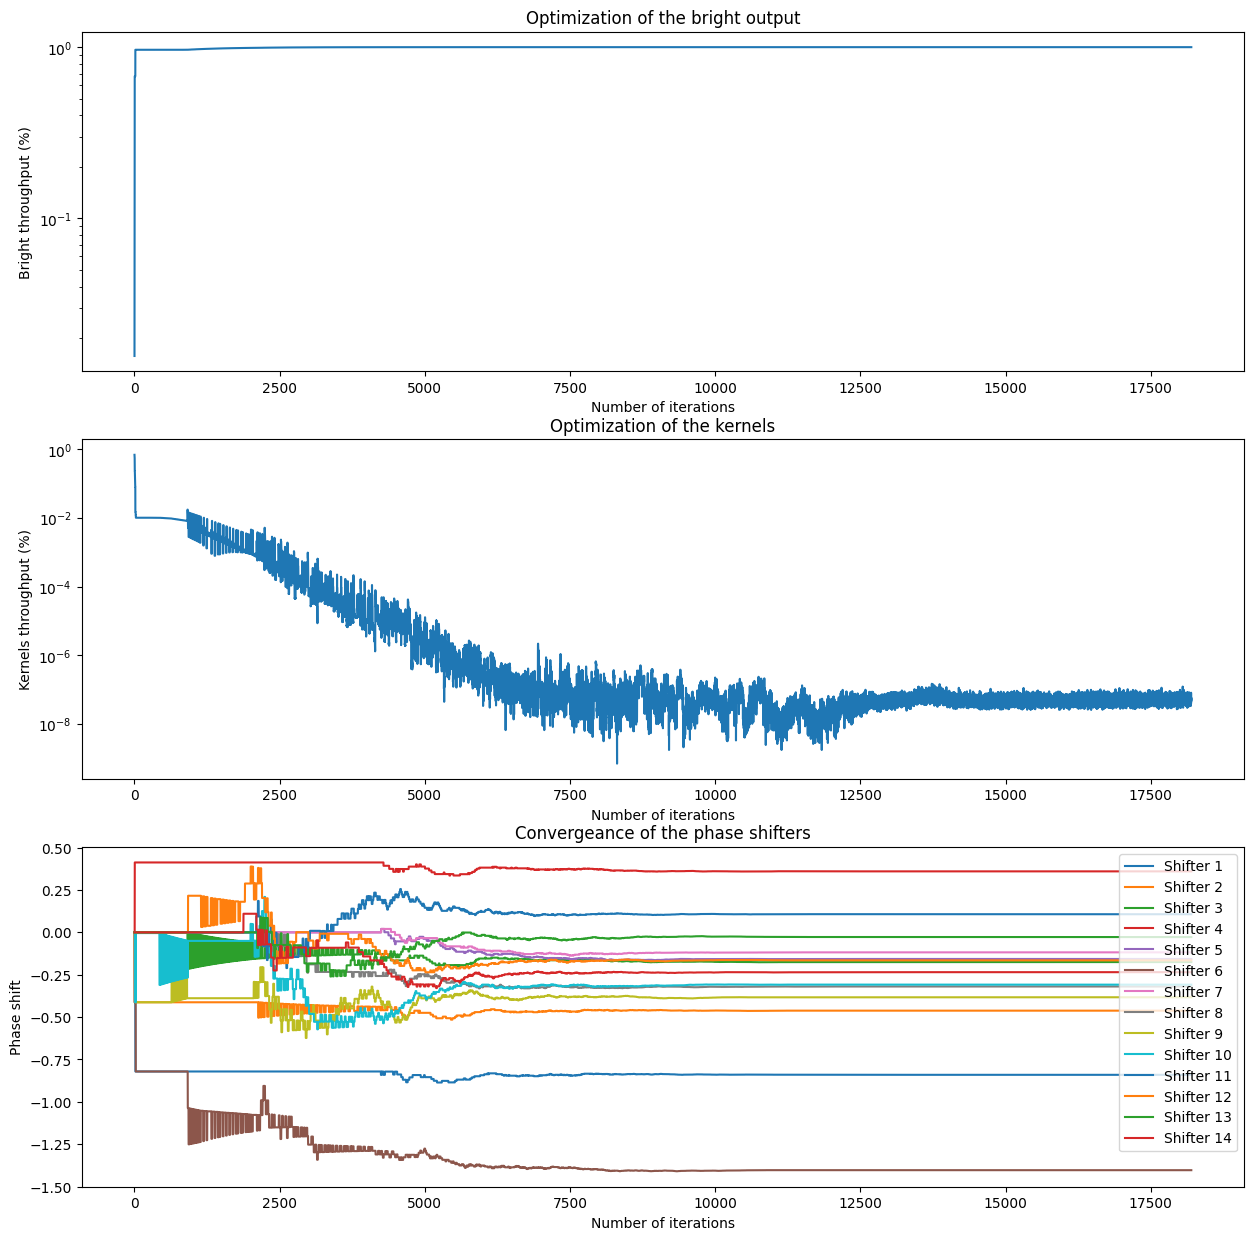
\includegraphics[height=7cm]{img/calibration_genetic.png}
                \end{tabular}
                \end{center}
                \caption[calibration_genetic] 
                { \label{fig:calibration_genetic} 
                Calibration using genetic algorithm [AJOUTER DESCRIPTION]}
            \end{figure}

        \subsubsection{Input obstruction}
            To overcome the limitations of the genetic algorithm, another calibration method has been implemented. This method is based on the principle of obstructing the component's inputs. We still inject a point source into the component but this time we obstruct 2 of its inputs. We then focus on one of its outputs whose transfer function is greatly simplified, to the point of having only one parameter (phase shifter) influencing this output.

            The algorithm is constructed as follows:

            \begin{enumerate}
                \item We obstruct inputs 3 and 4 then seek to maximize the bright output. Given that we are insensitive to the global phase, we can use the electric field phase of the first input as a reference phase. Thus, the bright output can be maximized by only adjusting phase shifter $P_2$.
                \item We obstruct inputs 1 and 2 then seek to maximize the bright output, this time by adjusting phase shifter $P_4$. We temporarily use the electric field phase of the third input as a reference phase.
                \item We obstruct inputs 2 and 4 then again seek to maximize the bright output. This time, we adjust phase shifter $P_3$, which will correspond to the phase difference at the output of the first layer of Nullers (Figure \ref{fig:architecture}). We then add the phase introduced on $P_3$ to that introduced on $P_4$ to change the common phase of $I_3$ and $I_4$.
                \item Still obstructing $I_2$ and $I_4$, we seek to minimize dark outputs 3 and 4 which are supposed to have inputs $I_1$ and $I_3$ in perfect phase opposition. For this, we adjust phase shifter $P_8$.
                \item We obstruct $I_3$ and $I_4$ and seek to minimize kernel 3. Given that the delays injected so far redirect the flux towards the bright output, we introduce a phase $+\frac{\pi}{2}$ on $P_2$, thus transforming the bright output into a dark output and the dark outputs associated with kernel 3 into bright outputs. We then adjust phase shifter $P_10$ to symmetrize the dark outputs (which we observe through the nulling of the kernel despite the presence of flux).
                \item Similarly, we obstruct $I_2$ and $I_4$ and seek to minimize kernel 2 by introducing a phase $+\frac{\pi}{2}$ on $P_3$. We then adjust phase shifter $P_10$.
                \item Finally, we obstruct $I_2$ and $I_3$ and seek to minimize kernel 1 by introducing a phase $+\frac{\pi}{2}$ on $P_4$. We then adjust phase shifter $P_9$.
            \end{enumerate}

            For each step, the correct phase to inject on the considered phase shifter can be obtained either dichotomously or formally by performing a series of measurements. Indeed, for each step, the problem simplifies sufficiently to be solved analytically. For example, for the first step, we seek to maximize the bright output $B$ which can then be written as:

            \begin{equation}
                B = \left|\left(a_1 e^{i(\theta_1 + \sigma_1 + \phi_1)} + a_2 e^{i(\theta_2 + \sigma_2 + \phi_2)}\right) e^{i(\sigma_5 + \phi_5)}\right|^2
            \end{equation}

            Where $a_n$ and $\theta_n$ represent the amplitude and phase of the input signals respectively. $\sigma_n$ corresponds to the (unknown) phase perturbation associated with shifter $n$ and $\phi_n$ is the phase that we voluntarily inject via the shifter to try to compensate for this perturbation.

            Since calibration is done in the laboratory, we can assume a total intensity fixed at $1$ (arbitrary unit) and that each input receives the same flux, i.e., $a_1 = a_2 = 1/\sqrt{2}$, and perfectly in phase, i.e., $\theta_1 = \theta_2 = \theta$. Since we only have access to signal intensity, we are insensitive to the global phase, which allows us to simplify the previous equation:

            \begin{equation}
                B = \frac{1}{2} \left|e^{i(\sigma_1 + \phi_1)} + e^{i(\sigma_2 + \phi_2)}\right|^2
            \end{equation}

            By maximizing $B$, we should then find $1$ which implies that

            \begin{equation}
                \sigma_1 + \phi_1 = \sigma_2 + \phi_2
            \end{equation}

            We can use $\phi_1$ as a reference (global phase) and thus fix it to 0, which then gives

            \begin{equation}
                \phi_2 = \sigma_1 - \sigma_2
            \end{equation}

            We can take different measurements of $B$ at fixed $\phi_2$ and deduce $\sigma_1$ and $\sigma_2$ by solving a system of equations.

            This second calibration method has the advantage of not suffering from photon noise sensitivity since we ensure at each step that we have flux on the outputs of interest. However, it is adapted to our architecture and must be completely rethought to be adapted to another Kernel-Nuller architecture. Moreover, it requires the action of moving parts to obstruct the component's inputs, which can be a disadvantage for automated calibration.

            Using this method, we numerically obtain a null depth also on the order of $10^{-8}$. Thanks to the successive simplification of the problem, we find ourselves in a case where convergence to an optimal solution is assured. [ADD LABORATORY RESULTS]

            \begin{figure}[H]
                \begin{center}
                \begin{tabular}{c}
                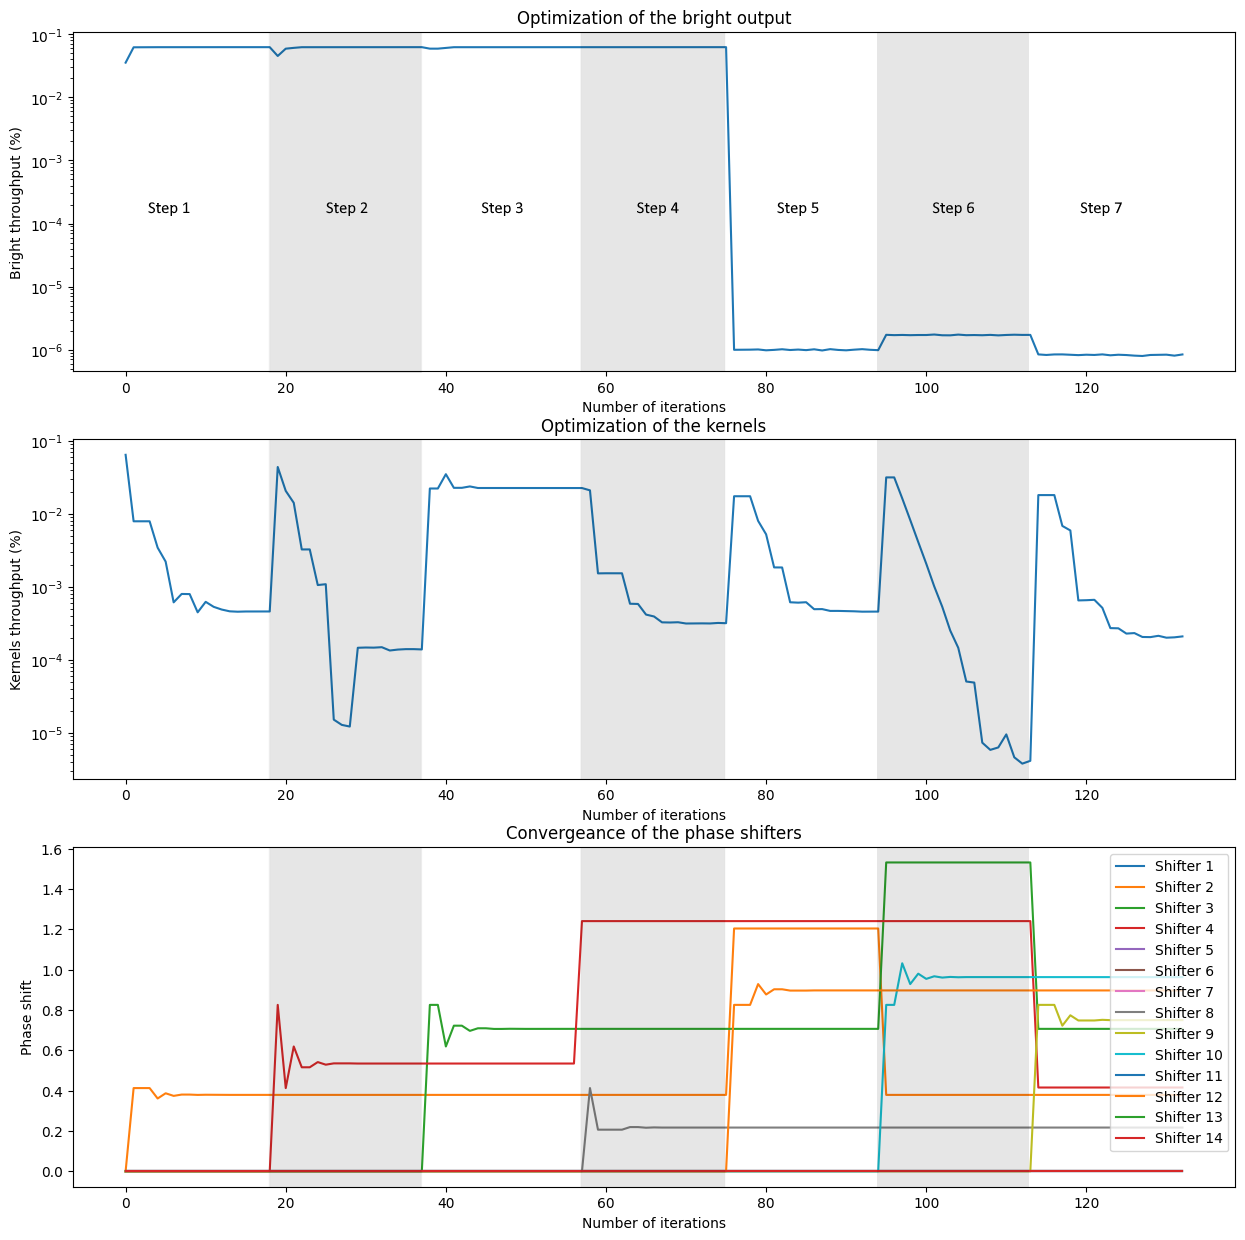
\includegraphics[height=7cm]{img/calibration_obstruction.png}
                \end{tabular}
                \end{center}
                \caption[calibration_obstruction] 
                { \label{fig:calibration_obstruction} 
                Calibration using input obstruction [AJOUTER DESCRIPTION]}
            \end{figure}

    \begin{figure}[H]
        \begin{center}
        \begin{tabular}{c}
        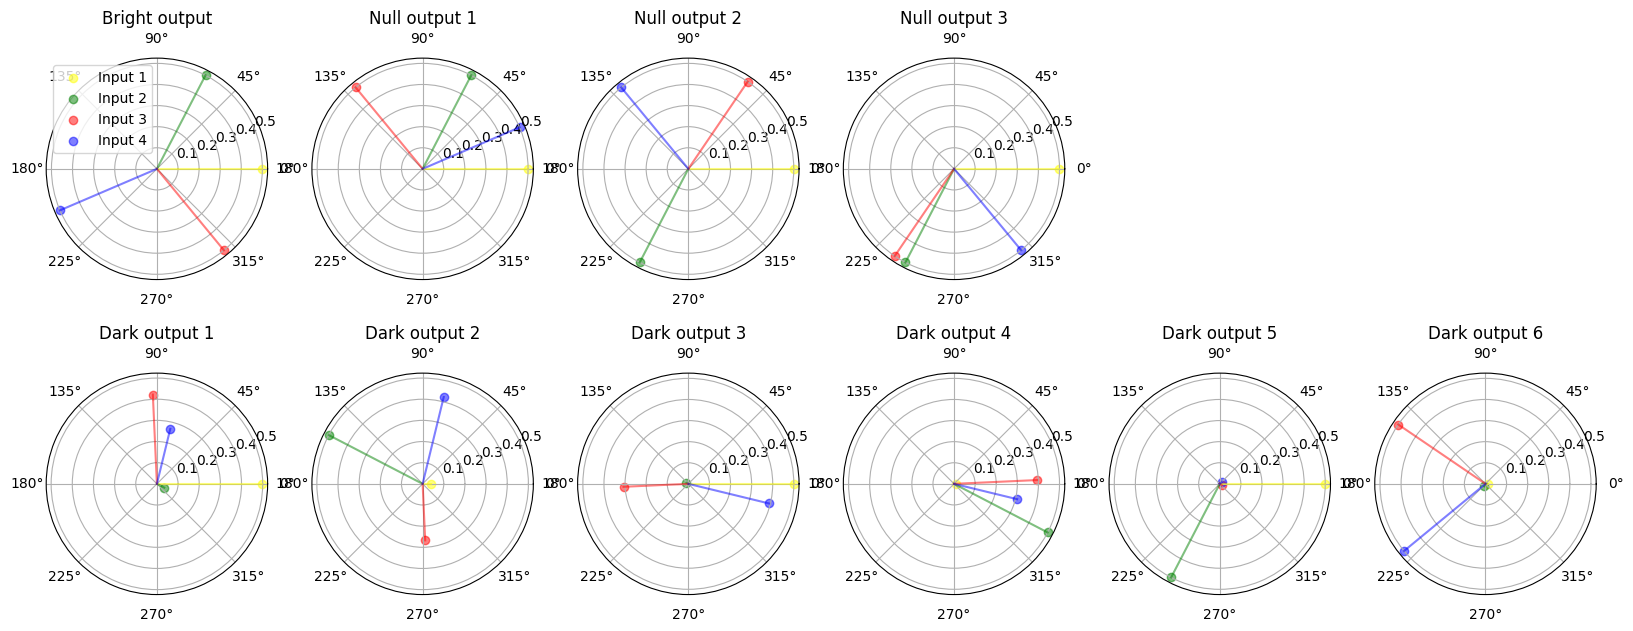
\includegraphics[height=3.2cm]{img/perturbed_phases.png}
        \end{tabular}
        \end{center}
        \caption[perturbed_phases] 
        { \label{fig:perturbed_phases} 
        Perturbed phases}
    \end{figure}

    \begin{figure}[H]
        \begin{center}
        \begin{tabular}{c}
        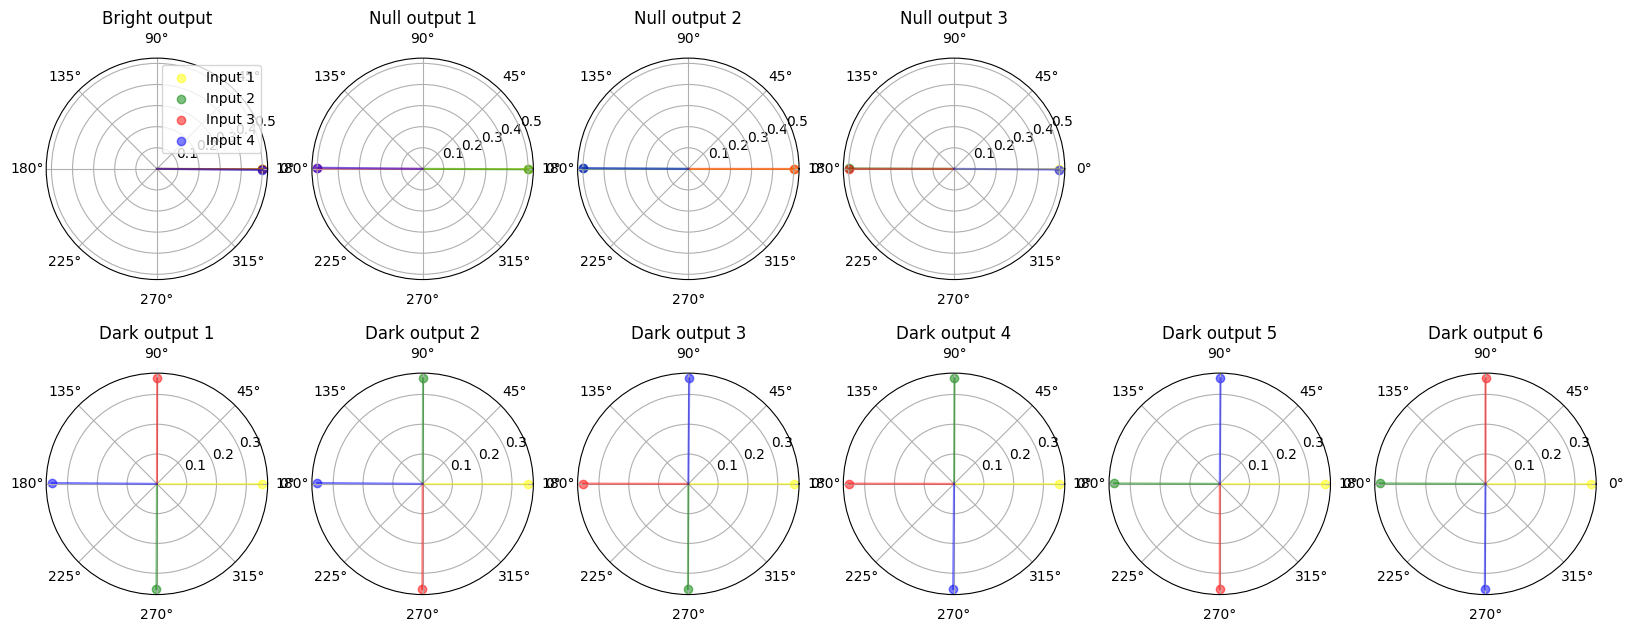
\includegraphics[height=3.2cm]{img/calibrated_phases.png}
        \end{tabular}
        \end{center}
        \caption[calibrated_phases] 
        { \label{fig:calibrated_phases} 
        Calibrated phases}
    \end{figure}

%--------------------------------------------------------------------

\section{Results and limitations}

    \begin{enumerate}
        \item Numerical results
        \subitem Kernel-Null depth (Fig \ref{fig:calibration_genetic} \& \ref{fig:calibration_obstruction})
        \subitem Kernel inversion and swapping 
        \item Laboratory results
        \item Laboratory limitations (ex. crosstalk)
    \end{enumerate}

    \begin{figure}[H]
        \begin{center}
        \begin{tabular}{c}
        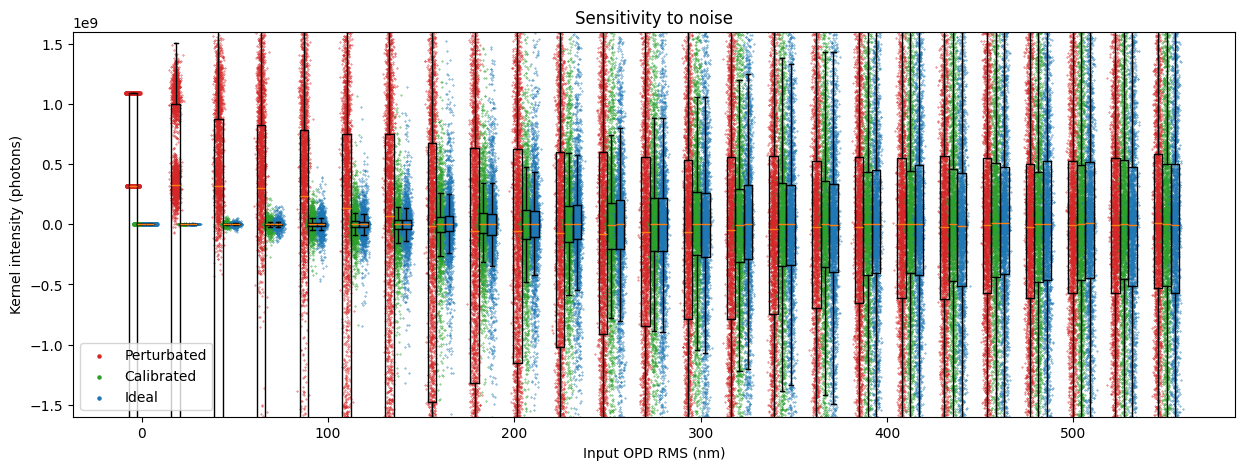
\includegraphics[height=3cm]{img/noise_sensitivity.png}
        \end{tabular}
        \end{center}
        \caption[noise_sensitivity] 
        { \label{fig:noise_sensitivity} 
        Sensitivity to input noise}
    \end{figure}

%-----------------------------------------------------------------

\section{Conclusions and prospects}

   \begin{enumerate}
      \item Conditions for noticing a performance gain
      \item Need of a post calibration caracterization process to identify the outputs
      \item Deeper statistical analysis is required to truely caracterize performance gain (the null depth is not the only relevant parameter)
      \item Architecture limitations (ex. no amplitude modulation, no photometric outputs)
   \end{enumerate}

\begin{acknowledgements}
      Lorem ipsum
\end{acknowledgements}

% WARNING
%-------------------------------------------------------------------
% Please note that we have included the references to the file aa.dem in
% order to compile it, but we ask you to:
%
% - use BibTeX with the regular commands:
%   \bibliographystyle{aa} % style aa.bst
%   \bibliography{Yourfile} % your references Yourfile.bib
%
% - join the .bib files when you upload your source files
%-------------------------------------------------------------------

\begin{thebibliography}{}

  \bibitem{lorem ipsum} Lorem ipsum

\end{thebibliography}

\end{document}
